%----------------------------------------------------------------------------
\section{AngularJS}
%----------------------------------------------------------------------------




Az AngularJS egy nyílt forrású JavaScript keretrendszer ami ``single-page''\footnote{Egy olyan webalkalmazás ami egy weboldalon kifér dinamikusan betöltött tartalommal a jobb felhasználói élmény céljából.} webalkalmazások fejlesztését támogatja. A Google karbantartása alatt van és az első verziója 2009-ben jelent meg. 

\subsection{Kliensoldali HTML generálás}

%\begin{figure}[!ht]
%\centering
%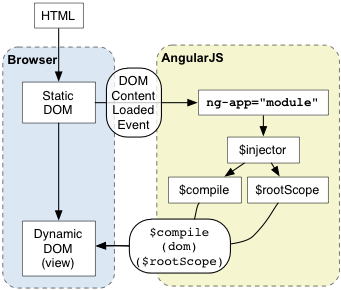
\includegraphics[width=10cm,keepaspectratio]{figures/concepts-startup.png}
%%\caption{Dinamikus kliensoldali HTML AngularJS-ben}
%\label{fig:angularhtml}
%\end{figure}

A hagyományos weboldal esetében a böngészőben megjelenített HTML a szerver oldali alkalmazás által van létrehozva.  A single-page alkalmazás ebben az esetben úgy jön létre, hogy AJAX felhasználásával betöltés után töltődnek be újabb részei az oldalnak \cite{angularbook}. AngularJS esetében ez a művelet a kliens oldalra kerül így a szerver inkább egy adatforrás és statikus tartalom szolgáltatóvá válik. Így lazább csatolást érünk el a szerver és kliens oldal között esetleg párhuzamosítva a fejlesztést és növelve az újrafelhasználhatóságot \cite{AngularDocConcepts}.





\subsection{Direktívák}

Az AngularJS fordító segítségével ki lehet terjeszteni a HTML szintaxist új attribútum és elem típusokkal, ezeket hívják direktívának. 

\lstset{language=HTML}
\begin{lstlisting}[frame=single]  
<ul>
  <li ng-repeat="action in user.actions">
    {{action.description}}
  </li>
</ul>
\end{lstlisting}

Magas szintről nézve a direktívák megjelölik a DOM elemeket és ennek hatására az AngularJS fordító speciális viselkedéssel bővíti ki ezeket az elemeket. A DOM-ot csak direktívák segítségével lehet befolyásolni AngularJS-ben és ez a szeparáció segít a tesztelésben. 

Beépített direktívák vannak, példáúl \lstinline{ng-repeat}, \lstinline{ng-click}, \lstinline{ng-show}, és ezek kiterjeszthetőek saját direktívákkal. Ekkor meg lehet határozni egy HTML templatet a direktívának, ami helyettesíti a DOM-ban a létező elemet az új template-tel és a direktíva \lstinline{link} attribútuma egy olyan függvény ami beállítja fordításkor a kiterjesztett viselkedést példáúl egy jQuery dátumkiválasztót kapcsol a DOM elemhez és ennek eseményeit hozzáköti a modellhez.


\subsection{Model-View-Controller}

Az MVC architektúra a desktop alkalmazások világában lett népszerű és csak az utóbbi években terjedt a webes alkalmazások világába. Az alap ötlet a tiszta elválasztása az adat kezelésnek (modell), az üzleti logikának (kontroller) és a megjelenítésnek (nézet). AngularJS alkalmazásokban a nézet a Document Object Model, a kontrollerek Javascript objektumok vagy függvények, és további objektum attribútumokban van tárolva a modell.   

\subsubsection{Adatkötés}

jQuery és hasonló megoldások segítségével újratöltés nélkül frissíteni tudjuk a DOM-ot felhasználói események hatására vagy adatok frissítése esetében, de még az egyszerű esetekben sem biztos hogy triviális a DOM és adatok összehangolása. Az AngularJS ezt két irányú adatkötéssel próbálja megoldani ráadásul deklaratívan. Egy egyszerű példa adatkötésre:

\lstset{language=HTML}
\begin{lstlisting}[frame=single]  
<div ng-controller="HelloController">
  <input ng-model="greeting.text"/>
  <p>{{greeting.text}}, World!</p>
</div>
\end{lstlisting}
Ekkor az input mező módosítása automatikusan a model-t is frissíti és ez a cimkét is frissíti alatta. Ehhez az alap funkcionalitáshoz nem is szükséges más kódot írni.


\subsubsection{Függőséginjektálás}

Függőséginjektálás egy szoftver tervezési minta amiben beégetett függőségek helyett kicserélhető komponenseket használunk amiket akár futás időben is cserélhetünk. 

Ez egység tesztelés esetében válik hasznossá, hiszen jobban lehet izolálni alkalmazás logikát azzal, hogy függőségeket kicserélünk a tesztekben egy úgynevezett ``mocked'' függőséggel. Egy jó példa olyan függőségre amit teszt esetekben ki szeretnénk cserélni egy olyan kódrészlet ami egy különálló rendszernek az API-ját használja ráadásul állapotmódosítással járó módon, amikor ezt ``mock-oljuk'', akkor tesztelni tudjuk az API felhasználását az API meghívása nélkül.

Egy kontroller a DOM -- vagy a nézet -- egy bizonyos részéhez van kötve, és függőséginjektálás során egy úgynevezett scope kontextus objektumhoz fér hozzá amin keresztül a modellhez férünk hozzá. Ez az elválasztás segít az újrafelhasználásban és karbantarthatóságban, mert, minden kontroller csak azt lát amit kell, hogy lásson és nem ``szennyezzük'' a globális környezetet. 

A scope objektumok egy hierarchiába vannak rendezve, létezik egy gyökér scope, és egymásbaágyazott kontrollerek scope objektumai prototípus örökléssel származnak egymásból.  
 
\begin{lstlisting}
function HelloController($scope) {
    $scope.greeting = {text: "Hello"}
}
\end{lstlisting}

\subsection{Szolgáltatások}

Az AngularJS szolgáltatások egyke példányok, amik bizonyos funkciót valósítanak meg az alkalmazásban, példáúl a \lstinline{http} szolgáltatás egy csomagoló a böngésző XMLHttpRequest objektuma körül és vele lehet AJAX hívásokat végrehajtani. 

AngularJS szolgáltatásokat injektálni kell, mint minden más függőséget, egy komponensbe, példáúl tudunk injektálni kontrollerbe, direktívába, szolgáltatásba stb. Természetesen saját szolgáltatást is lehet fejleszteni és ajánlott is az újrafelhasználandó logikát egy ilyen szolgáltatásba helyezni.

A kontrollerekbe mindig injektálni kell a \lstinline{scope} szolgáltatást, így megvalósul a kapcsolat a modell és a kontroller között.
